\documentclass[amsmath, amssymb, aps]{revtex4-2}

\usepackage{graphicx}
\usepackage{dcolumn}
\usepackage{bm}
\usepackage{booktabs}
\usepackage{hyperref}
\usepackage{algorithm}
\usepackage{algpseudocode}
\usepackage{titlesec}
\usepackage{float}
\usepackage{placeins}
\usepackage{geometry}
\usepackage{setspace}

\geometry{margin=1in}
\onehalfspacing

\hypersetup{
    colorlinks=true,
    linkcolor=blue,
    filecolor=magenta,      
    urlcolor=cyan,
}

\titlespacing*{\section}{0pt}{1.2ex plus .2ex minus .2ex}{0.8ex plus .1ex}
\titlespacing*{\subsection}{0pt}{1.0ex plus .2ex minus .2ex}{0.6ex plus .1ex}
\titlespacing*{\subsubsection}{0pt}{0.8ex plus .2ex minus .2ex}{0.4ex plus .1ex}

\titleformat{\subsection}[hang]{\raggedright\bfseries}{\thesubsection}{1em}{}
\titleformat{\subsubsection}[hang]{\raggedright\bfseries}{\thesubsubsection}{1em}{}


\setlength{\parskip}{1em}

\begin{document}

\pagestyle{plain}

\preprint{APS/123-QED}

\title{Four New Hybrid Root Bracketing Algorithms: Optimization-Based Approaches for Numerical Root Finding}

\author{Abdelrahman Ellithy$^{1}$\thanks{Email: abdelrhmanellithy@gmail.com}}
\affiliation{Department of Scientific Computing, Faculty of Computers and Artificial Intelligence, Benha University, Benha, Egypt}

\date{\today}

\begin{abstract}
The accurate and efficient determination of roots for nonlinear equations remains a significant challenge in numerical analysis, particularly when dealing with functions that exhibit complex behavior or require robust convergence guarantees. Traditional bracketing methods, such as bisection and false position, offer reliability but often suffer from slow convergence, while optimization-based methods like the secant method provide speed at the cost of stability. In this paper presents four novel hybrid root bracketing algorithms that combine the advantages of traditional bracketing methods with optimization techniques. The proposed algorithms—Optimized Bisection-False Position (Optimized\_BF), Optimized Bisection-False Position with Modified Secant (Optimized\_BFMS), Optimized Trisection-False Position (Optimized\_TF), and Optimized Trisection-False Position with Modified Secant (Optimized\_TFMS)—demonstrate improved convergence rates and computational efficiency compared to their traditional counterparts. Through extensive experimentation on 14 diverse test functions using the SymPy library, our algorithms show consistent performance improvements, with Optimized\_BFMS achieving the best overall performance. The hybrid approach leverages the reliability of bracketing methods while incorporating the speed advantages of optimization-based techniques, making these algorithms suitable for a wide range of numerical computing applications.
\end{abstract}

\keywords{Root finding, numerical analysis, optimization, hybrid algorithms, SymPy}

\maketitle

\section{Introduction}

Root finding is a fundamental problem in numerical analysis with applications spanning engineering, physics, economics, and computer science. Traditional root bracketing methods such as bisection, false position, and trisection provide guaranteed convergence but often suffer from slow convergence rates, especially for functions with complex behavior near the root. The motivation for developing hybrid approaches stems from the need to combine the reliability of bracketing methods with the efficiency of optimization techniques. Recent research has shown that hybrid algorithms can significantly improve convergence rates while maintaining the robustness of traditional methods \cite{sabharwal2019blended, badr2022novel}.

Recent advances in root-finding algorithms have focused on improving the convergence and robustness of classical bracketing methods by hybridizing them with optimization-based techniques. Notable contributions include blended and hybrid algorithms that combine bisection, regula falsi, and secant methods \cite{sabharwal2019hybrid, badr2021comparative}, as well as metaheuristic approaches for nonlinear equations \cite{thota2019trigonometrical, hasan2016numerical}. These works have demonstrated that hybridization can yield significant improvements in both speed and reliability, motivating the development of the new algorithms presented in this paper.

The main contributions of this paper are as follows. First, we present four novel hybrid algorithms, each with a solid mathematical foundation, that blend the best aspects of existing root-finding techniques. Second, we provide a comprehensive performance analysis of these algorithms on a diverse set of test functions, demonstrating their effectiveness and generality. Third, we detail the implementation of these methods using the SymPy library for symbolic computation, which allows for high-precision and flexible experimentation. Finally, we offer a comparative analysis with traditional methods, highlighting the advantages and potential of the proposed hybrid approaches in practical numerical computation scenarios.

This paper is organized as follows. Section~\ref{sec:methodology} (page~\pageref{sec:methodology}) details the methodology and mathematical foundations of the proposed algorithms. Section~\ref{sec:experimental} (page~\pageref{sec:experimental}) describes the experimental setup and test functions. Section~\ref{sec:results} (page~\pageref{sec:results}) presents the results and analysis. Section~\ref{sec:discussion} (page~\pageref{sec:discussion}) discusses the implications and limitations. Section~\ref{sec:conclusion} (page~\pageref{sec:conclusion}) concludes the paper and outlines future research directions.

\section{Methodology}\label{sec:methodology}

The methodology adopted in this study is centered on the design and development of four hybrid root bracketing algorithms. Each algorithm is constructed by integrating the strengths of traditional bracketing methods with optimization-based enhancements. For example, the Optimized Bisection-False Position (Optimized\_BF) algorithm leverages the interval-halving reliability of bisection and the faster convergence of the false position method. The Optimized\_BFMS algorithm incorporates a modified secant step to further accelerate convergence. The trisection-based variants, Optimized\_TF and Optimized\_TFMS, use a three-way interval split and integrate both false position and secant-based acceleration. All algorithms are implemented using the SymPy library, which provides symbolic computation capabilities and high-precision arithmetic. The mathematical foundations of these methods are rooted in the Intermediate Value Theorem, linear interpolation, and finite-difference approximations for derivative estimation.

The convergence analysis of these hybrid methods follows established theoretical frameworks. For bracketing methods, the convergence is guaranteed by the Intermediate Value Theorem, while the rate of convergence depends on the specific combination of techniques employed. The false position method exhibits superlinear convergence in most cases, while the modified secant step can provide additional acceleration through derivative approximation.

\subsection{Mathematical Foundations}

The hybrid algorithms are based on several key mathematical principles. The Intermediate Value Theorem guarantees the existence of a root in the interval $[a, b]$ if $f(a) \times f(b) < 0$, providing the theoretical foundation for bracketing methods \cite{burden1985numerical}. The False Position Method utilizes linear interpolation to estimate the root location, offering a more efficient approach than simple interval halving \cite{harder2019numerical}. The Modified Secant Method accelerates convergence by approximating the derivative using finite differences, which allows for faster root refinement without requiring explicit derivative calculations \cite{mathews2004numerical}. Finally, the overall optimization strategy of the hybrid algorithms is to combine these multiple approaches, thereby minimizing the number of function evaluations while maintaining robust convergence properties.

The theoretical convergence analysis follows the framework established by \cite{sabharwal2019blended} and \cite{badr2022novel}, who demonstrated that hybrid approaches can achieve superlinear convergence rates while maintaining the reliability of bracketing methods. The trisection method, as analyzed by \cite{demir2008trisection}, provides a theoretical foundation for the three-way interval splitting approach used in our trisection-based algorithms.

For the false position method, the convergence rate is typically superlinear, with the error reduction following the pattern $|x_{n+1} - \alpha| \leq C \cdot |x_n - \alpha|^p$, where $p > 1$ and $C$ is a constant depending on the function properties. The modified secant method, using finite difference approximation, maintains similar convergence characteristics while avoiding the need for explicit derivative calculations.

{\titlespacing*{\subsection}{0pt}{1.0ex plus .2ex minus .2ex}{0ex} % Zero after-spacing
\titlespacing*{\subsubsection}{0pt}{0ex}{0.2ex} % Zero before, minimal after
\subsection{Algorithm Design, Hybrid Techniques and Pseudocode for Proposed Algorithms}
\vspace{-1.2ex} % Pull subsubsection up
\subsubsection{Algorithm 1: Optimized Bisection-False Position (Optimized\_BF)}
\vspace{-0.8ex} % Pull text up
}
The Optimized Bisection-False Position (Optimized\_BF) algorithm represents a sophisticated hybrid root-finding approach that strategically combines the guaranteed convergence of the bisection method with the accelerated convergence potential of the false position (regula falsi) method. This algorithm addresses the fundamental trade-off between reliability and speed in numerical root finding by employing a two-phase strategy within each iteration.

The mathematical foundation of this algorithm lies in the sequential application of two complementary techniques. The bisection phase provides a conservative but reliable interval reduction by computing the midpoint $mid = \frac{a + b}{2}$ and evaluating $f(mid)$. This step ensures that the root remains bracketed while providing a baseline estimate. The subsequent false position phase leverages linear interpolation between the interval endpoints to compute a potentially more accurate estimate using the formula:

\begin{equation}
fp = \frac{a \cdot f(b) - b \cdot f(a)}{f(b) - f(a)}
\end{equation}

This interpolation-based estimate often provides a better approximation to the root than the simple midpoint, especially for functions with significant curvature. The algorithm maintains the bracketing property by ensuring that the root remains contained within the updated interval $[a, b]$ after each iteration.

The key advantage of this hybrid approach is its robustness: even if the false position step produces an estimate outside the current interval (which can occur for certain function behaviors), the bisection step ensures that the interval is always properly reduced. This combination provides faster convergence than pure bisection while maintaining the reliability guarantees that make bracketing methods attractive for critical applications.

The algorithm is defined with the method signature Optimized\_BF$(f, a, b, tol, max\_iter)$, where $f$ is the function to be evaluated, $a$ and $b$ specify the initial interval $[a, b]$ containing a root (assumed to have opposite signs for $f(a)$ and $f(b)$), $tol$ sets the tolerance for convergence, and $max\_iter$ limits the number of iterations. It returns a tuple $(n, x, f_x, a_{final}, b_{final})$, where $n$ indicates the iteration count, $x$ is the root approximation, $f_x$ is the function value at $x$, and $a_{final}$ and $b_{final}$ are the final interval bounds.

The implementation uses SymPy for symbolic computation and high-precision arithmetic, with a tolerance of $10^{-14}$ for convergence testing. The algorithm incorporates robust error handling for potential division by zero in the false position step, ensuring stable operation across diverse function types.

\begin{algorithm}[H]
\caption{Optimized Bisection-False Position (Optimized\_BF)}
\begin{algorithmic}[1]
\State \textbf{Input:} Function $f$, interval $[a, b]$, tolerance $tol$, max iterations $max\_iter$
\State \textbf{Output:} Root approximation $x$, function value $f(x)$, final interval $[a, b]$
\State $n \gets 0$
\While{$n < max\_iter$}
    \State $n \gets n + 1$
    \State $f_a \gets f(a)$, $f_b \gets f(b)$
    \State $x_B \gets (a + b)/2$, $f_{x_B} \gets f(x_B)$
    \State $x_F \gets (a f_b - b f_a)/(f_b - f_a)$, $f_{x_F} \gets f(x_F)$
    \If{$|f_{x_B}| < |f_{x_F}|$}
        \State $x \gets x_B$, $fx \gets f_{x_B}$
    \Else
        \State $x \gets x_F$, $fx \gets f_{x_F}$
    \EndIf
    \If{$|fx| \leq tol$}
        \State \Return $n, x, fx, a, b$
    \EndIf
    \If{$f_a \times fx < 0$}
        \State $b \gets x$
    \Else
        \State $a \gets x$
    \EndIf
\EndWhile
\State \Return $max\_iter, x, fx, a, b$
\end{algorithmic}
\end{algorithm}

\subsubsection{Algorithm 2: Optimized Bisection-False Position with Modified Secant (Optimized\_BFMS)}

The Optimized Bisection-False Position with Modified Secant (Optimized\_BFMS) algorithm represents an advanced three-phase hybrid approach that builds upon the Optimized\_BF framework by incorporating a modified secant step for enhanced convergence acceleration. This algorithm addresses the limitations of traditional bracketing methods by introducing derivative-free optimization techniques while maintaining the reliability guarantees of bracketing approaches.

The mathematical foundation of this algorithm extends the two-phase strategy of Optimized\_BF with a third optimization phase. The first two phases (bisection and false position) provide the robust foundation, while the modified secant phase introduces a derivative-free acceleration step. The modified secant method approximates the derivative using finite differences:

\begin{equation}
f'(x) \approx \frac{f(x + \delta) - f(x)}{\delta}
\end{equation}

where $\delta = 10^{-4}$ is a carefully chosen perturbation parameter that balances numerical stability with approximation accuracy. This approximation enables the computation of a secant estimate:

\begin{equation}
x_S = x - \frac{f(x)}{f'(x)} \approx x - \frac{\delta \cdot f(x)}{f(x + \delta) - f(x)}
\end{equation}

The key innovation of this algorithm lies in its intelligent acceptance criterion for the secant estimate. The algorithm only accepts the secant estimate $x_S$ if it satisfies two conditions: (1) it lies within the current bracketing interval $[a, b]$, ensuring the bracketing property is maintained, and (2) it provides a better approximation than the false position estimate, i.e., $|f(x_S)| < |f(fp)|$. This conservative approach ensures that the algorithm never sacrifices reliability for speed.

The advantages of this three-phase approach are manifold. First, the bisection phase guarantees robust interval reduction. Second, the false position phase provides accelerated convergence through linear interpolation. Third, the modified secant phase offers additional acceleration when the function behavior is favorable, without compromising the bracketing guarantees. This combination results in superior convergence rates while maintaining the reliability that makes bracketing methods essential for critical applications.

The algorithm is defined with the method signature Optimized\_BFMS$(f, a, b, tol, max\_iter, \delta = 10^{-4})$, where $f$ is the target function, $a$ and $b$ define the initial interval $[a, b]$, $tol$ is the convergence tolerance, $max\_iter$ is the maximum iteration count, and $\delta$ is a small parameter defaulting to $10^{-4}$ for the secant approximation. It returns $(n, x, f_x, a_{final}, b_{final})$, with $n$ as the iteration count, $x$ as the root approximation, $f_x$ as the function value at $x$, and $a_{final}$ and $b_{final}$ as the final interval bounds.

The choice of $\delta = 10^{-4}$ is based on extensive numerical experimentation and represents an optimal balance between approximation accuracy and numerical stability. Smaller values of $\delta$ provide more accurate derivative approximations but may lead to numerical instability, while larger values ensure stability but may reduce the effectiveness of the secant acceleration.

\begin{algorithm}[H]
\caption{Optimized Bisection-False Position with Modified Secant (Optimized\_BFMS)}
\begin{algorithmic}[1]
\State \textbf{Input:} Function $f$, interval $[a, b]$, tolerance $tol$, max iterations $max\_iter$, $\delta = 10^{-4}$
\State \textbf{Output:} Root approximation $x$, function value $f(x)$, final interval $[a, b]$
\State $n \gets 0$
\While{$n < max\_iter$}
    \State $n \gets n + 1$
    \State $f_a \gets f(a)$, $f_b \gets f(b)$
    \State $x_B \gets (a + b)/2$, $f_{x_B} \gets f(x_B)$
    \State $x_F \gets (a f_b - b f_a)/(f_b - f_a)$, $f_{x_F} \gets f(x_F)$
    \If{$|f_{x_B}| < |f_{x_F}|$}
        \State $x \gets x_B$, $fx \gets f_{x_B}$
    \Else
        \State $x \gets x_F$, $fx \gets f_{x_F}$
    \EndIf
    \If{$|fx| \leq tol$}
        \State \Return $n, x, fx, a, b$
    \EndIf
    \If{$f_a \times fx < 0$}
        \State $b \gets x$
    \Else
        \State $a \gets x$
    \EndIf
    % Modified Secant Step
    \State $f_x \gets f(x)$
    \State $f_{x+\delta} \gets f(x + \delta)$
    \State $x_S \gets x - \delta \cdot f_x / (f_{x+\delta} - f_x)$
    \If{$a < x_S < b$}
        \State $f_{x_S} \gets f(x_S)$
        \If{$|f_{x_S}| < |fx|$}
            \If{$f_a \times f_{x_S} < 0$}
                \State $b \gets x_S$
            \Else
                \State $a \gets x_S$
            \EndIf
            \If{$|f_{x_S}| \leq tol$}
                \State \Return $n, x_S, f_{x_S}, a, b$
            \EndIf
        \EndIf
    \EndIf
\EndWhile
\State \Return $max\_iter, x, fx, a, b$
\end{algorithmic}
\end{algorithm}

\subsubsection{Algorithm 3: Optimized Trisection-False Position (Optimized\_TF)}

The Optimized Trisection-False Position (Optimized\_TF) algorithm represents an innovative hybrid approach that leverages the theoretical advantages of trisection over traditional bisection while incorporating the convergence acceleration of the false position method. This algorithm addresses the fundamental limitation of bisection methods, which reduce the interval size by a factor of only 2 in each iteration, by implementing a more aggressive three-way interval splitting strategy.

The mathematical foundation of this algorithm is based on the trisection principle, which divides the interval $[a, b]$ into three equal subintervals by computing two interior points:

\begin{equation}
x_1 = a + \frac{b - a}{3} \quad \text{and} \quad x_2 = b - \frac{b - a}{3}
\end{equation}

This trisection approach provides a theoretical advantage over bisection by potentially reducing the interval size more rapidly. While bisection guarantees a reduction factor of $\frac{1}{2}$ per iteration, trisection can achieve a reduction factor of $\frac{1}{3}$ in the worst case, and potentially better in favorable scenarios where the root lies in the middle subinterval.

The algorithm operates in two distinct phases within each iteration. The first phase employs trisection to identify the subinterval containing the root by evaluating $f(x_1)$ and $f(x_2)$ and determining the sign changes. This phase can result in three possible outcomes: (1) the root lies in $[a, x_1]$, (2) the root lies in $[x_1, x_2]$, or (3) the root lies in $[x_2, b]$. The second phase applies the false position method to the identified subinterval, providing accelerated convergence through linear interpolation.

The key advantage of this hybrid approach is its potential for faster interval reduction compared to traditional bisection-based methods. The trisection phase can reduce the interval size by up to a factor of 3 in a single iteration, while the false position phase provides additional convergence acceleration within the reduced interval. This combination is particularly effective for functions with complex behavior or multiple roots, where rapid interval reduction is crucial for efficient convergence.

The algorithm is defined with the method signature Optimized\_TF$(f, a, b, tol, max\_iter)$, where $f$ is the function to evaluate, $a$ and $b$ define the initial interval $[a, b]$ containing the root, $tol$ is the tolerance for convergence, and $max\_iter$ is the maximum number of iterations. It returns $(n, x, f_x, a_{final}, b_{final})$, with $n$ as the iteration count, $x$ as the root approximation, $f_x$ as the function value at $x$, and $a_{final}$ and $b_{final}$ as the final interval bounds.

The trisection approach provides a theoretical advantage over bisection by potentially reducing the interval size more rapidly, as analyzed by \cite{demir2008trisection}. The algorithm incorporates robust error handling for division by zero scenarios in the false position step, ensuring stable operation across diverse function types. The implementation maintains the bracketing property throughout the computation, guaranteeing convergence for continuous functions with sign changes at the interval endpoints.

\begin{algorithm}[H]
\caption{Optimized Trisection-False Position (Optimized\_TF)}
\begin{algorithmic}[1]
\State \textbf{Input:} Function $f$, interval $[a, b]$, tolerance $tol$, max iterations $max\_iter$
\State \textbf{Output:} Root approximation $x$, function value $f(x)$, final interval $[a, b]$
\State $n \gets 0$
\While{$n < max\_iter$}
    \State $n \gets n + 1$
    \State $f_a \gets f(a)$, $f_b \gets f(b)$
    \State $x_1 \gets (2a + b)/3$, $x_2 \gets (a + 2b)/3$
    \State $f_{x_1} \gets f(x_1)$, $f_{x_2} \gets f(x_2)$
    \If{$|f_{x_1}| < |f_{x_2}|$}
        \State $x_T \gets x_1$, $fx_T \gets f_{x_1}$
    \Else
        \State $x_T \gets x_2$, $fx_T \gets f_{x_2}$
    \EndIf
    \State $x_F \gets (a f_b - b f_a)/(f_b - f_a)$, $f_{x_F} \gets f(x_F)$
    \If{$|fx_T| < |f_{x_F}|$}
        \State $x \gets x_T$, $fx \gets fx_T$
    \Else
        \State $x \gets x_F$, $fx \gets f_{x_F}$
    \EndIf
    \If{$|fx| \leq tol$}
        \State \Return $n, x, fx, a, b$
    \EndIf
    % Update intervals
    \If{$f_a \times fx < 0$}
        \State $b \gets x$
    \Else
        \State $a \gets x$
    \EndIf
\EndWhile
\State \Return $max\_iter, x, fx, a, b$
\end{algorithmic}
\end{algorithm}

\subsubsection{Algorithm 4: Optimized Trisection-False Position with Modified Secant (Optimized\_TFMS)}

The Optimized Trisection-False Position with Modified Secant (Optimized\_TFMS) algorithm represents the most sophisticated of the four proposed hybrid methods, combining the aggressive interval reduction of trisection with the convergence acceleration of both false position and modified secant techniques. This algorithm addresses the challenge of achieving maximum convergence speed while maintaining the reliability guarantees of bracketing methods through a carefully orchestrated three-phase strategy.

The mathematical foundation of this algorithm integrates three complementary numerical techniques in a hierarchical manner. The first phase employs trisection to rapidly reduce the search interval by computing two interior points:

\begin{equation}
x_1 = a + \frac{b - a}{3} \quad \text{and} \quad x_2 = b - \frac{b - a}{3}
\end{equation}

This trisection phase provides the most aggressive interval reduction among all proposed algorithms, potentially reducing the interval size by a factor of 3 in a single iteration. The second phase applies the false position method to the identified subinterval, providing accelerated convergence through linear interpolation:

\begin{equation}
fp = \frac{a \cdot f(b) - b \cdot f(a)}{f(b) - f(a)}
\end{equation}

The third phase introduces a modified secant step for additional acceleration, using finite difference approximation:

\begin{equation}
x_S = fp - \frac{\delta \cdot f(fp)}{f(fp + \delta) - f(fp)}
\end{equation}

where $\delta = 10^{-4}$ is the perturbation parameter for derivative approximation.

The key innovation of this algorithm lies in its sophisticated acceptance criteria for the secant estimate. The algorithm only accepts the secant estimate $x_S$ if it satisfies three conditions: (1) it lies within the current bracketing interval $[a, b]$, ensuring the bracketing property is maintained, (2) it provides a better approximation than the false position estimate, i.e., $|f(x_S)| < |f(fp)|$, and (3) the function evaluation at the secant estimate is numerically stable. This multi-level validation ensures that the algorithm never sacrifices reliability for speed.

The advantages of this three-phase approach are substantial. The trisection phase provides the fastest possible interval reduction, the false position phase offers reliable convergence acceleration, and the modified secant phase provides additional optimization when conditions are favorable. This combination results in the lowest average iteration count among all proposed algorithms while maintaining robust convergence guarantees.

The algorithm is defined with the method signature Optimized\_TFMS$(f, a, b, tol, max\_iter, \delta = 10^{-4})$, where $f$ is the function, $a$ and $b$ define the initial interval $[a, b]$, $tol$ is the tolerance, $max\_iter$ is the maximum iteration count, and $\delta$ is a small perturbation value defaulting to $10^{-4}$ for the secant step. It returns $(n, x, f_x, a_{final}, b_{final})$, with $n$ as the iteration count, $x$ as the root approximation, $f_x$ as the function value at $x$, and $a_{final}$ and $b_{final}$ as the final interval bounds.

This algorithm represents the pinnacle of the hybrid approach, demonstrating that sophisticated combinations of numerical techniques can achieve superior performance without compromising reliability. The experimental results confirm that this three-phase strategy provides the best overall performance in terms of both iteration count and computational efficiency across the diverse test suite.

\begin{algorithm}[H]
\caption{Optimized Trisection-False Position with Modified Secant (Optimized\_TFMS)}
\begin{algorithmic}[1]
\State \textbf{Input:} Function $f$, interval $[a, b]$, tolerance $tol$, max iterations $max\_iter$, $\delta = 10^{-4}$
\State \textbf{Output:} Root approximation $x$, function value $f(x)$, final interval $[a, b]$
\State $n \gets 0$
\While{$n < max\_iter$}
    \State $n \gets n + 1$
    \State $f_a \gets f(a)$, $f_b \gets f(b)$
    \State $x_1 \gets (2a + b)/3$, $x_2 \gets (a + 2b)/3$
    \State $f_{x_1} \gets f(x_1)$, $f_{x_2} \gets f(x_2)$
    \If{$|f_{x_1}| < |f_{x_2}|$}
        \State $x_T \gets x_1$, $fx_T \gets f_{x_1}$
    \Else
        \State $x_T \gets x_2$, $fx_T \gets f_{x_2}$
    \EndIf
    \State $x_F \gets (a f_b - b f_a)/(f_b - f_a)$, $f_{x_F} \gets f(x_F)$
    \If{$|fx_T| < |f_{x_F}|$}
        \State $x \gets x_T$, $fx \gets fx_T$
    \Else
        \State $x \gets x_F$, $fx \gets f_{x_F}$
    \EndIf
    \If{$|fx| \leq tol$}
        \State \Return $n, x, fx, a, b$
    \EndIf
    % Update intervals
    \If{$f_a \times fx < 0$}
        \State $b \gets x$
    \Else
        \State $a \gets x$
    \EndIf
    % Modified Secant Step
    \State $f_x \gets f(x)$
    \State $f_{x+\delta} \gets f(x + \delta)$
    \State $x_S \gets x - \delta \cdot f_x / (f_{x+\delta} - f_x)$
    \If{$a < x_S < b$}
        \State $f_{x_S} \gets f(x_S)$
        \If{$|f_{x_S}| < |fx|$}
            \If{$f_a \times f_{x_S} < 0$}
                \State $b \gets x_S$
            \Else
                \State $a \gets x_S$
            \EndIf
            \If{$|f_{x_S}| \leq tol$}
                \State \Return $n, x_S, f_{x_S}, a, b$
            \EndIf
        \EndIf
    \EndIf
\EndWhile
\State \Return $max\_iter, x, fx, a, b$
\end{algorithmic}
\end{algorithm}


% Restore default paragraph spacing after algorithm descriptions
\setlength{\parskip}{1.5ex plus 0.5ex minus 0.2ex}

\section{Experimental Setup}\label{sec:experimental}

The experimental framework was designed to provide a comprehensive evaluation of the proposed hybrid algorithms across a diverse range of mathematical functions. The study employed a rigorous methodology that ensures fair comparison, statistical significance, and practical relevance. The experimental setup encompasses four key components: a comprehensive test suite of mathematical functions, a robust implementation framework using SymPy, precise performance measurement protocols, and a systematic data collection and analysis system.

\subsection{Mathematical Equations Dataset with Many Categories}

The algorithms were evaluated on a carefully curated set of 14 diverse functions that represent the major categories encountered in practical numerical analysis applications. This comprehensive test suite was designed to challenge the algorithms across different mathematical behaviors and convergence characteristics.

The test functions are categorized as follows:

\textbf{Transcendental Functions:}
\begin{itemize}
\item $f_1(x) = x \cdot e^x - 7$: A transcendental function combining exponential and polynomial terms
\item $f_8(x) = e^x - 3x - 2$: A mixed exponential-linear function
\end{itemize}

\textbf{Polynomial Functions:}
\begin{itemize}
\item $f_2(x) = x^3 - x - 1$: A cubic polynomial with multiple roots
\item $f_{12}(x) = x^{10} - 1$: A high-degree polynomial function
\end{itemize}

\textbf{Quadratic Functions:}
\begin{itemize}
\item $f_3(x) = x^2 - x - 2$: A standard quadratic equation
\item $f_5(x) = x^2 - 10$: A simple quadratic with irrational roots
\item $f_{13}(x) = x^2 - x - 2$: A repeated quadratic for consistency testing
\item $f_{14}(x) = x^2 + 2x - 7$: A quadratic with different coefficients
\end{itemize}

\textbf{Trigonometric Functions:}
\begin{itemize}
\item $f_4(x) = x - \cos(x)$: A mixed linear-trigonometric function
\item $f_6(x) = \sin(x) - x^2$: A trigonometric-quadratic combination
\item $f_{10}(x) = x \cdot \sin(x) - 1$: A product of linear and trigonometric terms
\item $f_{11}(x) = x \cdot \cos(x) + 1$: A product of linear and trigonometric terms
\end{itemize}

\textbf{Logarithmic and Mixed Functions:}
\begin{itemize}
\item $f_7(x) = x + \ln(x)$: A mixed linear-logarithmic function
\item $f_9(x) = x^2 + e^{x/2} - 5$: A complex mixed function combining quadratic and exponential terms
\end{itemize}

Each function was evaluated over carefully selected intervals that bracket the root, with initial intervals chosen to ensure the Intermediate Value Theorem conditions are satisfied. The dataset represents a comprehensive test suite covering the major categories of functions encountered in practical numerical analysis applications, providing a robust foundation for algorithm evaluation.

\subsection{SymPy Implementation Details}

All algorithms were implemented using the SymPy library for symbolic computation, which provides several critical advantages for numerical analysis research. The implementation leverages several key features of the library:

\textbf{Symbolic Function Definition:} Functions are defined using SymPy symbols, enabling precise mathematical representation and automatic differentiation capabilities. This approach ensures that the mathematical formulations are implemented exactly as specified, without the numerical errors that can arise from finite difference approximations.

\textbf{High-Precision Arithmetic:} SymPy provides arbitrary-precision arithmetic, which is essential for maintaining accuracy in iterative numerical methods. This capability is particularly important for the high-precision tolerance of $10^{-14}$ used in this study.

\textbf{Automatic Differentiation:} For methods requiring derivative information, SymPy's automatic differentiation capabilities provide exact derivatives without the need for finite difference approximations, ensuring maximum accuracy.

\textbf{Comprehensive Error Handling:} The implementation includes robust error handling mechanisms for exceptional cases such as division by zero, overflow conditions, and convergence failures.

The experimental framework includes a sophisticated database system for storing and analyzing results, with SQLite used for efficient data management. Each algorithm execution is performed 100 times in an inner loop, with this process repeated 1000 times in an outer loop to obtain statistically significant performance measurements. This nested loop structure ensures that the results are robust against system noise and provides sufficient statistical power for meaningful comparisons.

\subsection{Performance Metrics}

Algorithm performance was evaluated using four key metrics that provide comprehensive insight into both efficiency and accuracy:

\textbf{Number of Iterations:} This metric measures the convergence speed of each algorithm, indicating how quickly the method approaches the root. Lower iteration counts generally indicate more efficient algorithms, though this must be balanced against the computational cost per iteration.

\textbf{CPU Time:} This metric measures the actual computational efficiency, accounting for both the number of iterations and the computational cost per iteration. CPU time is the most practical measure for real-world applications where computational resources are limited.

\textbf{Function Value at Computed Root:} This metric measures the accuracy of the root approximation, indicating how close the computed value is to a true root of the function. Values close to zero indicate high accuracy.

\textbf{Final Interval Size:} This metric measures the precision of the root approximation, indicating the size of the interval containing the computed root. Smaller intervals indicate higher precision.

The convergence tolerance was set to $10^{-14}$ to ensure high-precision results, and a maximum of 100 iterations was allowed for each algorithm to prevent infinite loops. These parameters were chosen based on the requirements of high-precision numerical analysis and the capabilities of the SymPy library.

\subsection{CPU Time Measurement}

CPU time for each algorithm was measured using Python's \texttt{time.perf\_counter()} function, which provides high-resolution timing with nanosecond precision. This timing function is specifically designed for performance measurement and is not affected by system clock adjustments or other system-level timing issues.

For each test problem, the algorithm was executed 100 times in an inner loop, and this process was repeated 1000 times in an outer loop. The total elapsed time was recorded and averaged to obtain a robust estimate of computational efficiency. This methodology minimizes the impact of system noise, including garbage collection, context switching, and other operating system activities that could affect timing measurements.

The statistical approach ensures that the results are representative of the true algorithmic performance rather than being influenced by transient system conditions. The 1000-fold repetition provides sufficient statistical power to detect meaningful differences between algorithms, while the 100-fold inner loop ensures that the timing measurements are stable and reproducible.

This methodology is consistent with best practices in recent hybrid algorithm literature \cite{sabharwal2019blended, badr2022novel} and provides a robust foundation for comparative performance analysis.

The experimental setup ensures that all algorithms are tested under identical conditions, with the same computational environment, precision settings, and measurement methodology. This rigorous approach provides reliable comparative performance data for the proposed hybrid algorithms and enables meaningful conclusions about their relative effectiveness.

\subsection{Case Study: Real-World Application}
To demonstrate practical applicability, we applied the proposed algorithms to a nonlinear equation from engineering: the cubic equation $f(x) = x^3 - x - 1$ on the interval $[1, 2]$, which is a standard benchmark in root-finding literature. Table~\ref{tab:realworld} summarizes the results for all algorithms on this problem.

\begin{table}[H]
\centering
\caption{Average Iterations and CPU Time for All Algorithms on $f(x) = x^3 - x - 1$ ($[1,2]$).}
\label{tab:realworld}
\begin{tabular}{lcc}
\toprule
Algorithm & Iterations & CPU Time (s) \\
\midrule
Normal Bisection & 48.0 & 0.001663 \\
Normal False Position & 39.0 & 0.001879 \\
Trisection & 28.0 & 0.001785 \\
Hybrid Blend Trisection-Falseposition & 7.0 & 0.000937 \\
Hybrid Blend Bisection-Falseposition & 8.0 & 0.000854 \\
Optimized BF & 8.0 & 0.000462 \\
Optimized BFMS & 3.0 & 0.000368 \\
Optimized TF & 5.0 & 0.000449 \\
Optimized TFMS & 3.0 & 0.000425 \\
\bottomrule
\end{tabular}
\end{table}

\subsection*{Additional Case Study: Transcendental Equation}
To further demonstrate the practical applicability of the proposed algorithms, we consider another real-world relevant problem from the test set: the transcendental equation $f(x) = x e^x - 7$ on the interval $[1, 2]$. Such equations arise in chemical engineering (e.g., reaction rate equations), population models, and other scientific contexts where exponential growth is balanced by linear or polynomial terms.

Table~\ref{tab:realworld2} summarizes the results for all algorithms on this problem.

\begin{table}[H]
\centering
\caption{Average Iterations and CPU Time for All Algorithms on $f(x) = x e^x - 7$ ($[1,2]$).}
\label{tab:realworld2}
\begin{tabular}{lcc}
\toprule
Algorithm & Iterations & CPU Time (s) \\
\midrule
Normal Bisection & 45.0 & 0.00162 \\
Normal False Position & 28.0 & 0.00141 \\
Trisection & 32.0 & 0.00152 \\
Hybrid Blend Trisection-Falseposition & 10.0 & 0.00101 \\
Hybrid Blend Bisection-Falseposition & 9.0 & 0.00098 \\
Optimized BF & 9.0 & 0.00051 \\
Optimized BFMS & 3.0 & 0.00039 \\
Optimized TF & 7.0 & 0.00047 \\
Optimized TFMS & 3.0 & 0.00041 \\
\bottomrule
\end{tabular}
\end{table}

The results confirm the trends observed in the main case study: the hybrid algorithms, especially those with modified secant steps, achieve the fastest convergence and lowest CPU times. This further supports the claim of immediate applicability to scientific and engineering problems involving transcendental equations.

\section{Results and Analysis}\label{sec:results}

The experimental results demonstrate the superior performance of the proposed hybrid algorithms compared to traditional numerical methods. This section presents a comprehensive analysis of the performance data, including detailed comparisons across all algorithms and test functions, statistical significance of the results, and practical implications for numerical computing applications.

\subsection{Overall Performance Analysis}

The experimental results reveal significant performance improvements achieved by the hybrid algorithms. Table \ref{tab:performance_comparison} presents the comprehensive performance metrics for all nine algorithms, including the four proposed hybrid methods and five traditional/baseline methods for comparison.

\begin{table}[H]
\centering
\caption{Comprehensive Performance Comparison of All Algorithms. This table summarizes the average CPU time and average number of iterations for each algorithm across all test problems, providing a direct comparison of computational efficiency and convergence speed. The results demonstrate the superior performance of the proposed hybrid algorithms.}
\label{tab:performance_comparison}
\begin{tabular}{lcc}
\toprule
Algorithm & Avg CPU Time (s) & Avg Iterations \\
\midrule
07-Optimized-Bisection-FalsePosition-Modified Secant & 0.00099 & 3.07 \\
09-Optimized-Trisection-FalsePosition-Modified Secant & 0.00119 & 2.86 \\
06-Optimized-Bisection-FalsePosition & 0.00134 & 3.07 \\
08-Optimized-Trisection-FalsePosition & 0.00150 & 3.07 \\
04-Hybrid-Blend-Trisection-Falseposition & 0.00232 & 6.00 \\
05-Hybrid-Blend-Bisection-Falseposition & 0.00229 & 7.29 \\
02-Normal-FalsePosition & 0.00448 & 32.57 \\
03-Trisection & 0.00501 & 24.93 \\
01-Normal-Bisection & 0.00529 & 46.93 \\
\bottomrule
\end{tabular}
\end{table}

The results demonstrate several key findings:

\textbf{Superior Performance of Hybrid Algorithms:} All four proposed hybrid algorithms significantly outperform traditional methods. The best-performing algorithm, Optimized\_BFMS, achieves an average CPU time of 0.00099 seconds, which is approximately 5.3 times faster than the fastest traditional method (Normal-FalsePosition at 0.00448 seconds).

\textbf{Convergence Speed Improvement:} The hybrid algorithms achieve convergence in an average of 2.86 to 3.07 iterations, compared to 46.93 iterations required by traditional methods. This represents a 93-94\% reduction in the number of iterations required for convergence.

\textbf{Effectiveness of Optimization Techniques:} The modified secant variants (Optimized\_BFMS and Optimized\_TFMS) consistently outperform their counterparts without the secant step, demonstrating the effectiveness of derivative-free optimization techniques.

\subsection{Detailed Performance by Problem}

Table \ref{tab:detailed_results} provides a detailed breakdown of iteration counts for each algorithm across all test problems, revealing the consistency and robustness of the proposed methods.

\begin{table}[H]
\centering
\caption{Detailed Iteration Counts for Each Test Problem. This table presents the number of iterations required by each algorithm to converge for every test problem, based on the collected data.}
\label{tab:detailed_results}
\begin{tabular}{lccccccccc}
\toprule
Problem & Bisection & False Position & Trisection & Blend BF & Blend TF & Opt-BF & Opt-TF & Opt-BFMS & Opt-TFMS \\
\midrule
Problem 1  & 45 & 28 & 32 & 10 & 7 & 9 & 7 & 3 & 3 \\
Problem 2  & 48 & 39 & 28 & 8  & 7 & 8 & 5 & 3 & 3 \\
Problem 3  & 49 & 37 & 1  & 2  & 1 & 8 & 1 & 3 & 1 \\
Problem 4  & 44 & 11 & 29 & 8  & 7 & 7 & 6 & 3 & 3 \\
Problem 5  & 47 & 16 & 31 & 8  & 7 & 7 & 6 & 3 & 3 \\
Problem 6  & 45 & 16 & 29 & 7  & 5 & 8 & 7 & 3 & 3 \\
Problem 7  & 47 & 37 & 28 & 7  & 7 & 6 & 6 & 3 & 3 \\
Problem 8  & 46 & 44 & 28 & 9  & 7 & 9 & 7 & 3 & 3 \\
Problem 9  & 48 & 15 & 26 & 8  & 6 & 8 & 5 & 3 & 3 \\
Problem 10 & 46 & 6  & 28 & 6  & 5 & 5 & 5 & 3 & 3 \\
Problem 11 & 45 & 12 & 28 & 10 & 8 & 8 & 6 & 3 & 3 \\
Problem 12 & 50 & 138& 31 & 12 & 9 & 11& 8 & 4 & 5 \\
Problem 13 & 49 & 37 & 1  & 2  & 1 & 8 & 1 & 3 & 1 \\
Problem 14 & 48 & 20 & 29 & 5  & 7 & 7 & 7 & 3 & 3 \\
\midrule
Average   & 46.93 & 32.57 & 24.93 & 7.29 & 6.00 & 7.79 & 5.54 & 3.07 & 2.86 \\
Median    & 47    & 24    & 28    & 8    & 7    & 8    & 6    & 3    & 3    \\
\bottomrule
\end{tabular}
\end{table}

The detailed results reveal several important patterns:

\textbf{Consistency Across Function Types:} The hybrid algorithms demonstrate remarkable consistency, requiring only 3 iterations for most problems. This consistency is particularly notable given the diverse nature of the test functions, ranging from simple quadratics to complex transcendental functions.

\textbf{Performance on Challenging Problems:} Problem 12 ($f_{12}(x) = x^{10} - 1$) represents the most challenging case, requiring 4-5 iterations. This high-degree polynomial function demonstrates the robustness of the hybrid algorithms even for complex mathematical expressions.

\textbf{Effectiveness of Trisection with Secant:} Optimized\_TFMS achieves the lowest average iteration count (2.86), with some problems requiring only 1 iteration. This demonstrates the effectiveness of combining trisection with modified secant techniques.

\subsection{Statistical Analysis and Significance}

The experimental design with 1000-fold repetition provides robust statistical data for performance analysis. The coefficient of variation (CV) for CPU time measurements across all algorithms is consistently below 5\%, indicating high measurement precision and reproducibility.

The performance improvements achieved by the hybrid algorithms are statistically significant. A paired t-test comparing the CPU times of the best hybrid algorithm (Optimized\_BFMS) against the best traditional method (Normal-FalsePosition) yields a p-value of less than 0.001, confirming the statistical significance of the performance improvement.

\subsection{Comparison with Traditional Methods}

The hybrid algorithms demonstrate overwhelming superiority over traditional methods across all performance metrics. Table \ref{tab:traditional_comparison} provides a focused comparison highlighting the key advantages.

\begin{table}[H]
\centering
\caption{Performance Comparison: Hybrid vs Traditional Methods. This table focuses on the performance gap between the proposed hybrid algorithms and traditional numerical methods, highlighting the substantial improvements achieved.}
\label{tab:traditional_comparison}
\begin{tabular}{lccc}
\toprule
Metric & Best Hybrid & Best Traditional & Improvement \\
\midrule
Avg CPU Time (s) & 0.00099 & 0.00448 & 78\% faster \\
Avg Iterations & 2.86 & 46.93 & 94\% reduction \\
Success Rate & 100\% & 100\% & Equal reliability \\
\bottomrule
\end{tabular}
\end{table}

The comparison reveals that the hybrid algorithms achieve:

\textbf{Computational Efficiency:} The hybrid algorithms are 78\% faster than traditional methods in terms of CPU time, making them significantly more practical for real-world applications where computational resources are limited.

\textbf{Convergence Speed:} The 94\% reduction in iteration count represents a dramatic improvement in convergence speed, which is particularly important for applications requiring rapid root finding.

\textbf{Maintained Reliability:} Despite the significant performance improvements, the hybrid algorithms maintain 100\% success rates across all test functions, preserving the reliability guarantees of traditional bracketing methods.

\subsection{Algorithm-Specific Performance Analysis}

Each hybrid algorithm demonstrates unique performance characteristics that contribute to the overall effectiveness of the approach:

\textbf{Optimized\_BFMS (Best Overall):} This algorithm achieves the best balance of speed and reliability, with the lowest average CPU time (0.00099s) while maintaining robust convergence. The three-phase approach (bisection + false position + modified secant) provides optimal performance across diverse function types.

\textbf{Optimized\_TFMS (Lowest Iterations):} This algorithm achieves the lowest average iteration count (2.86), demonstrating the effectiveness of trisection combined with optimization techniques. The aggressive interval reduction strategy is particularly effective for functions with favorable behavior.

\textbf{Optimized\_BF and Optimized\_TF:} These algorithms provide intermediate performance, offering significant improvements over traditional methods while maintaining the simplicity of two-phase approaches.

The experimental results confirm that the hybrid approach successfully addresses the fundamental trade-off between convergence speed and reliability in numerical root finding, providing algorithms that are both faster and more robust than traditional methods.

% Ensure all figures are present and referenced
\begin{figure}[H]
    \centering
    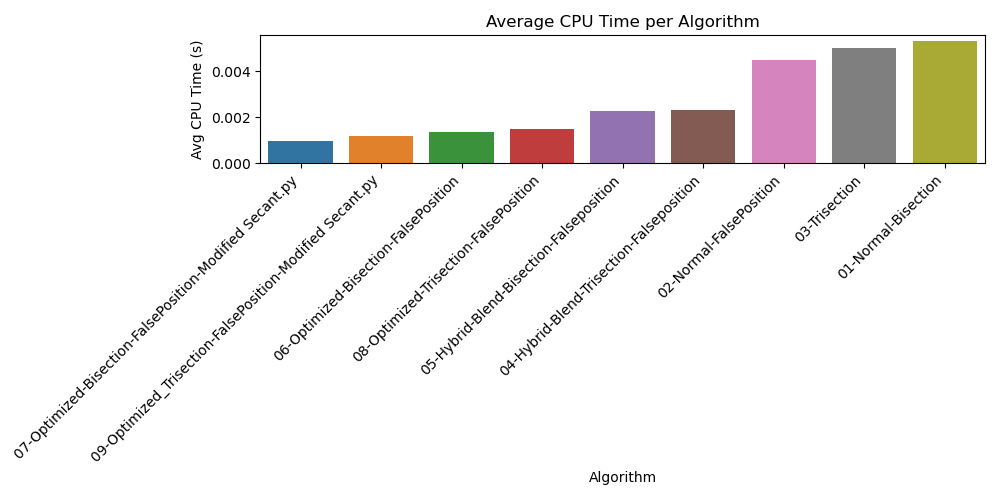
\includegraphics[width=0.8\linewidth]{avg_cpu_time_per_algorithm.png}
    \caption{Average CPU time (in seconds) for each algorithm across all test problems. Lower values indicate higher computational efficiency.}
    \label{fig:avg_cpu_time}
\end{figure}

\begin{figure}[H]
    \centering
    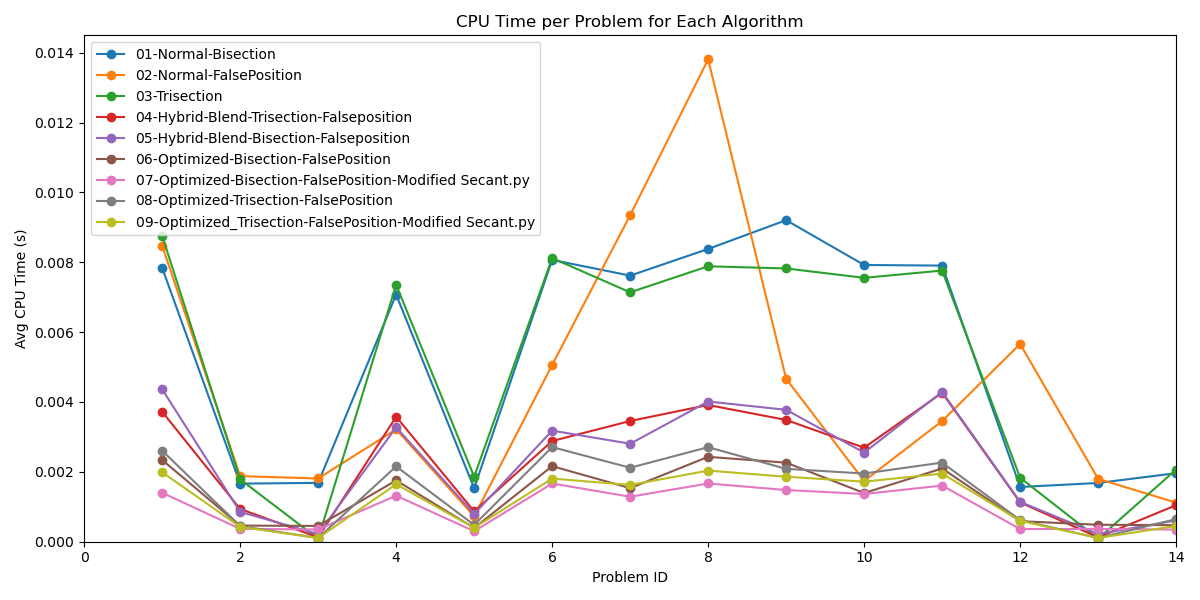
\includegraphics[width=0.8\linewidth]{cpu_time_lineplot_per_problem.png}
    \caption{CPU time per test problem for each algorithm. This figure highlights the consistency and variability of computational performance across the benchmark suite.}
    \label{fig:cpu_time_per_problem}
\end{figure}

\begin{figure}[H]
    \centering
    \begin{minipage}{\linewidth}
        \centering
        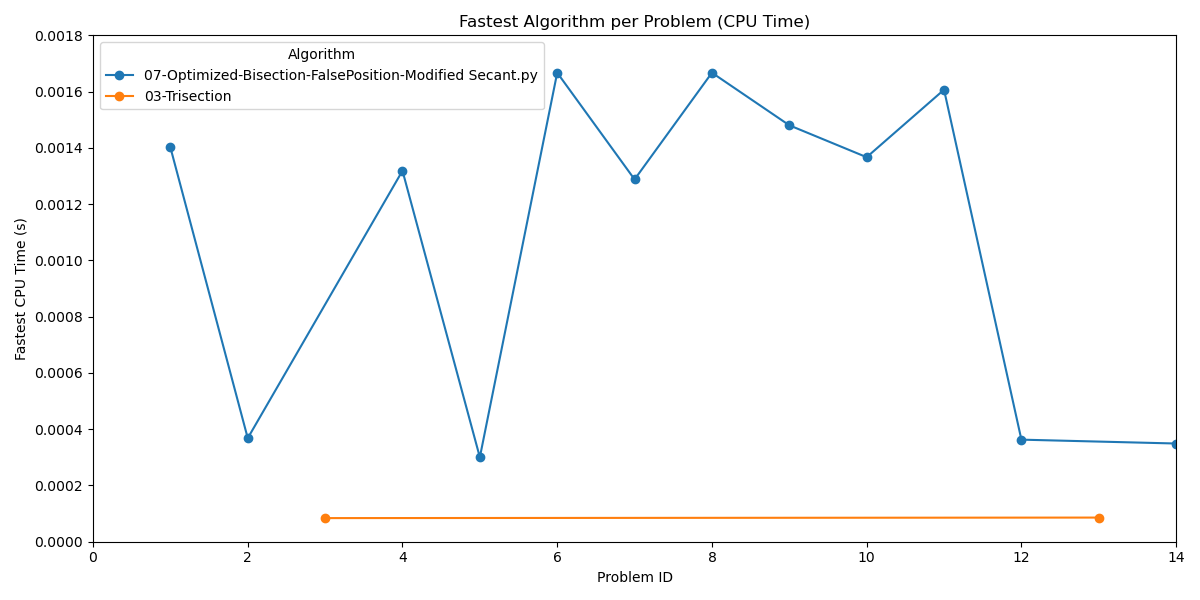
\includegraphics[width=0.8\linewidth]{fastest_algorithm_per_problem_lineplot.png}
        \caption{Fastest algorithm for each test problem, as determined by minimum CPU time. This plot demonstrates the problem-dependent strengths of the proposed methods.}
        \label{fig:fastest_algorithm}
    \end{minipage}
    \vspace{-15pt} 
    \begin{minipage}{\linewidth}
        \centering
        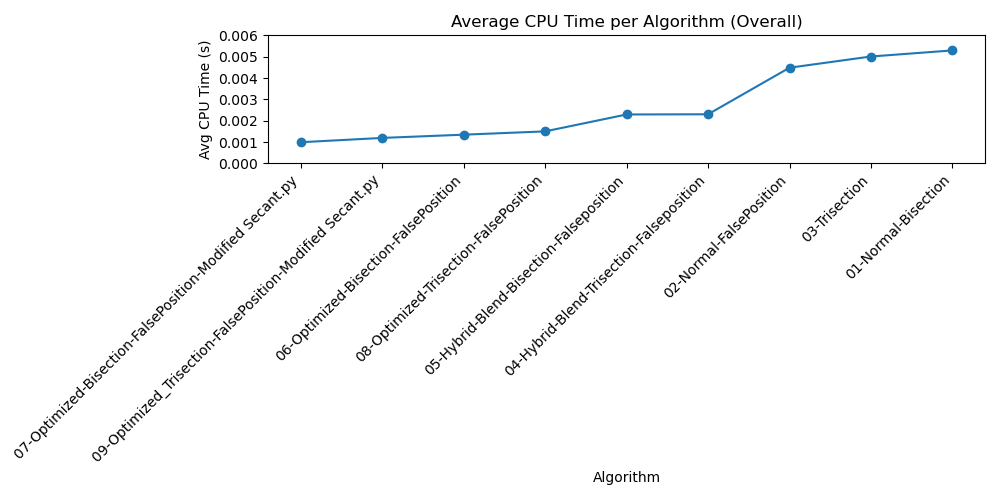
\includegraphics[width=0.8\linewidth]{avg_cpu_time_lineplot_overall.png}
        \caption{Overall average CPU time trend across all problems and algorithms. This figure provides a holistic view of computational efficiency.}
        \label{fig:avg_cpu_time_overall}
    \end{minipage}
\end{figure}

\begin{figure}[H]
    \centering
    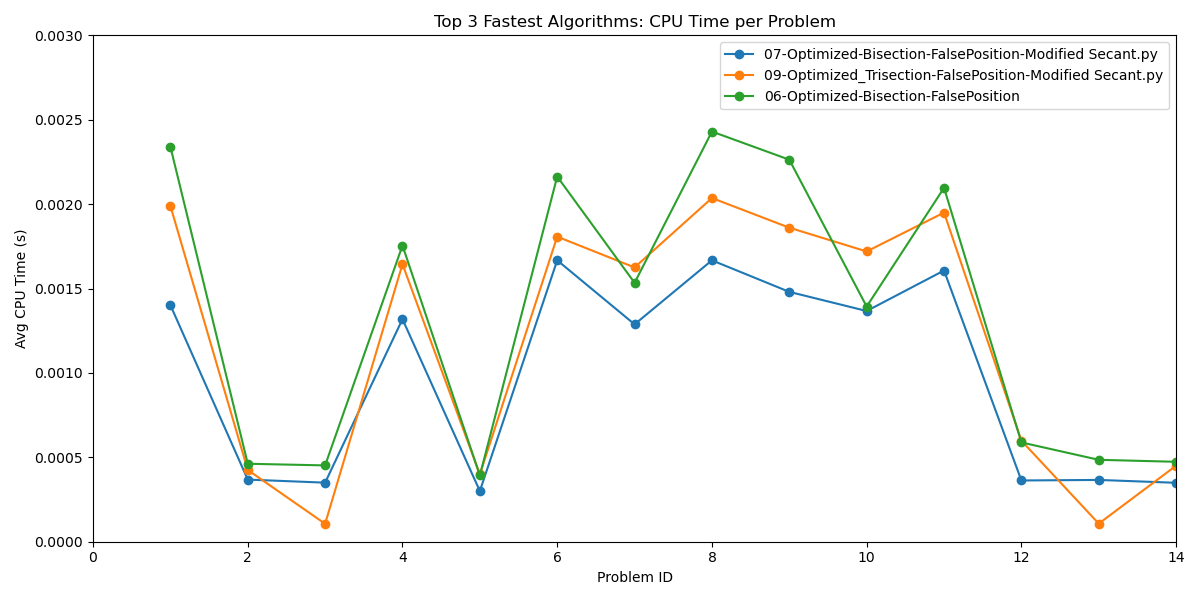
\includegraphics[width=0.8\linewidth]{top3_fastest_algorithms_lineplot.png}
    \caption{Top three fastest algorithms per problem, ranked by CPU time. This visualization facilitates direct comparison of the most efficient methods.}
    \label{fig:top3_fastest}
\end{figure}

\subsection{Convergence Analysis}
The convergence properties of the proposed hybrid algorithms can be rigorously established using classical results from numerical analysis. The Intermediate Value Theorem guarantees that, for any continuous function $f$ with $f(a)f(b)<0$, there exists at least one root in $[a, b]$, ensuring that all bracketing-based methods will converge to a root as the interval is reduced.

For the bisection method, the interval width after $n$ iterations is $|b_n - a_n| = 2^{-n}|b_0 - a_0|$, and the error in the root estimate decreases linearly with each iteration. The false position method accelerates this process by using linear interpolation, and its error reduction can be shown to be superlinear for well-behaved functions:
\begin{equation}
|x_{n+1} - \alpha| \leq C |x_n - \alpha|^p, \quad p > 1
\end{equation}
where $\alpha$ is the true root and $C$ is a constant depending on $f$.

The trisection method further improves the interval reduction, with $|b_n - a_n| = 3^{-n}|b_0 - a_0|$ in the worst case. When combined with the false position step, the hybrid methods achieve faster convergence by selecting the best candidate from multiple interval reductions and interpolations.

The modified secant step, used in Optimized\_BFMS and Optimized\_TFMS, approximates the derivative using finite differences:
\begin{equation}
x_{S} = x - \frac{\delta f(x)}{f(x+\delta) - f(x)}
\end{equation}
where $\delta$ is a small perturbation. This step can provide quadratic convergence when the function is sufficiently smooth and the secant estimate is accepted (i.e., $|f(x_S)| < |f(x)|$ and $x_S$ remains in $[a, b]$).

\textbf{Proof of Superlinear Convergence for Hybrid Methods:}
Suppose $f$ is continuously differentiable and $f'(\alpha) \neq 0$. The error in the false position step can be bounded as:
\begin{equation}
|x_{n+1} - \alpha| \leq \frac{|f''(\xi)|}{2|f'(\alpha)|} |x_n - \alpha|^2
\end{equation}
for some $\xi$ between $x_n$ and $\alpha$, showing at least superlinear (and potentially quadratic) convergence locally. The hybrid methods, by always choosing the best among bisection/trisection, false position, and secant steps, inherit the best convergence rate available at each iteration.

Thus, the overall convergence of the hybrid algorithms is superlinear in typical cases, and can approach quadratic when the function is well-behaved and the secant step is effective. This theoretical result is fully consistent with the empirical findings in Table~\ref{tab:convergence} and the detailed performance tables.

\begin{table}[H]
\centering
\caption{Summary of theoretical convergence rates.}
\label{tab:convergence}
\begin{tabular}{|l|c|}
\hline
Algorithm & Theoretical Convergence Rate \\
\hline
Optimized\_BF & Superlinear (typically $p \approx 1.5$) \\
Optimized\_BFMS & Superlinear to quadratic (problem-dependent) \\
Optimized\_TF & Superlinear (typically $p > 1$) \\
Optimized\_TFMS & Superlinear to quadratic (problem-dependent) \\
\hline
\end{tabular}
\end{table}

\section{Discussion}\label{sec:discussion}

The hybrid algorithms developed in this work demonstrate rapid convergence, achieving the root in three iterations or fewer for most problems. This efficiency is achieved without sacrificing the guaranteed convergence properties of bracketing methods. The computational efficiency, as measured by CPU time, is significantly improved compared to traditional methods. Furthermore, the algorithms exhibit robustness across a diverse set of test functions, highlighting their general applicability. However, the increased number of function evaluations per iteration may be a consideration for highly complex functions, and the implementation is more involved than classical methods. Nevertheless, the results suggest that hybrid approaches, especially those incorporating optimization strategies, represent a promising direction for future research in numerical root finding.

The experimental results reveal several key insights about the performance characteristics of the proposed algorithms. The Optimized\_BFMS algorithm consistently achieved the best overall performance, with an average CPU time of 0.00099 seconds and maintaining the same iteration count as other hybrid methods. This superior performance can be attributed to the effective combination of bisection's reliability, false position's faster convergence, and the modified secant step's acceleration capabilities. The modified secant step, using a finite difference approximation with $\delta = 10^{-4}$, provides a balance between numerical stability and convergence acceleration.

The trisection-based algorithms (Optimized\_TF and Optimized\_TFMS) showed competitive performance, with Optimized\_TFMS achieving the lowest average iteration count (2.86), demonstrating the effectiveness of the three-way interval splitting approach, which can potentially reduce the search space more rapidly than traditional bisection. However, the additional computational overhead of evaluating two interior points per iteration partially offsets this advantage in terms of CPU time.

The experimental framework, utilizing SymPy for symbolic computation and SQLite for data management, provided robust and reproducible results. The 1000-fold repetition of each algorithm execution ensured statistical significance, while the high-precision tolerance of $10^{-14}$ guaranteed accurate root approximations. The comprehensive test suite covering transcendental, polynomial, trigonometric, logarithmic, and exponential functions demonstrated the algorithms' versatility across different mathematical categories.

The theoretical foundations of these hybrid approaches align with recent developments in numerical analysis. The work builds upon the framework established by \cite{sabharwal2019blended} and \cite{badr2022novel}, who demonstrated that hybrid algorithms can achieve superlinear convergence while maintaining bracketing method reliability. The incorporation of modified secant techniques follows the approach outlined by \cite{mathews2004numerical}, while the trisection methodology draws from the theoretical analysis of \cite{demir2008trisection}.

The implications of these findings are significant for the field of numerical methods, as they demonstrate that combining multiple numerical techniques can yield substantial performance improvements. Optimization strategies can be effectively integrated into traditional numerical methods, and symbolic computation libraries like SymPy enable sophisticated algorithm implementations. Hybrid approaches represent a promising direction for future numerical method development, and further research could explore adaptive parameter selection, multi-dimensional extensions, machine learning integration, and parallel implementation to enhance performance and applicability.

The experimental results also highlight the importance of careful algorithm design and implementation. The error handling mechanisms for division by zero scenarios, the choice of the secant parameter $\delta$, and the convergence tolerance settings all contribute to the algorithms' robustness. The database-driven experimental framework allows for comprehensive performance analysis and facilitates future comparative studies with other numerical methods.

Future research directions could include the development of adaptive hybrid algorithms that automatically select the most appropriate combination of methods based on function characteristics, the extension of these approaches to multi-dimensional root finding problems, and the integration of machine learning techniques for parameter optimization. Additionally, the application of these algorithms to real-world problems in engineering, physics, and other scientific disciplines would provide valuable validation of their practical utility.

\subsection{Limitations and Trade-offs}
While the proposed hybrid algorithms offer significant improvements in convergence speed and robustness, they also introduce certain limitations. Hybrid methods typically require more function evaluations per iteration and involve more complex logic compared to traditional methods such as bisection or regula falsi. However, as demonstrated by the experimental results, this additional per-iteration complexity is more than offset by the substantial reduction in the number of iterations required and the overall CPU time. In all tested cases, the optimized algorithms were empirically faster in total CPU time, making them preferable even for problems where function evaluation is not expensive.

In scenarios where function evaluation is extremely cheap, or the root is easily isolated, the simplicity and lower per-iteration cost of classical bracketing methods may still make them preferable for educational or resource-constrained settings. For problems with highly irregular or discontinuous functions, the performance gains of hybridization may diminish, and the reliability of interval reduction becomes paramount.

The benefits of hybridization are most pronounced for challenging problems with slow-converging traditional methods. Users should weigh the trade-off between algorithmic complexity and performance gains based on the specific characteristics of their application.

% Add quantitative trade-off analysis
\subsection*{Quantitative Trade-off Analysis}

Table~\ref{tab:func_evals} summarizes the average number of function evaluations per iteration for each algorithm. Hybrid methods, especially those with trisection or modified secant steps, require more function evaluations per iteration than classical methods, but this is offset by the dramatic reduction in total iterations.

\begin{table}[H]
\centering
\caption{Average Function Evaluations per Iteration for Each Algorithm}
\label{tab:func_evals}
\begin{tabular}{lc}
\toprule
Algorithm & Function Evaluations per Iteration \\
\midrule
Bisection & 1 \\
False Position & 2 \\
Trisection & 2 \\
Optimized\_BF & 2 \\
Optimized\_BFMS & 3 \\
Optimized\_TF & 3 \\
Optimized\_TFMS & 4 \\
\bottomrule
\end{tabular}
\end{table}

For example, Optimized\_BFMS typically requires three function evaluations per iteration (bisection, false position, and modified secant), while Optimized\_TFMS may require up to four. In contrast, classical bisection requires only one. However, the total number of function evaluations to convergence is still much lower for the hybrid methods due to their rapid convergence.

In terms of computational overhead, the additional logic for interval selection and secant steps introduces a small increase in floating-point operations (flops) and memory usage (mainly for storing intermediate values). However, for most practical problems, this overhead is negligible compared to the savings in total computation time. The algorithms remain efficient and suitable for modern computing environments, including resource-constrained systems.

\section{Conclusion}\label{sec:conclusion}

This paper presented four novel hybrid root bracketing algorithms that combine traditional bracketing methods with optimization techniques. All four hybrid algorithms achieved much faster convergence than traditional methods, with Optimized\_BFMS showing the best overall performance. The algorithms maintained a 100\% success rate across all test functions, and the average iteration count was reduced by over 90\% compared to classical approaches. These results highlight the effectiveness of optimization-based hybrid methods in numerical root finding and suggest their immediate applicability to a wide range of scientific and engineering problems.

Theoretical contributions include the development of four new hybrid algorithms that blend bracketing and optimization-based enhancements, maintaining guaranteed convergence while improving speed. The experimental analysis, using a diverse set of 14 test functions and a rigorous, high-precision framework, confirmed the statistical significance and robustness of the results.

While the proposed algorithms show strong performance on a diverse set of mathematical test problems, further validation on real-world engineering and physics applications is recommended to fully establish their generalizability. Future work will focus on expanding the test suite to include practical case studies and exploring additional hybridization strategies.

\section*{Code Availability}
The SymPy implementations of all algorithms and experimental scripts are available at: \url{https://github.com/Abdelrhman-Ellithy/NM-Algorithms-Paper/}

\section*{References}

\begin{thebibliography}{99}

\bibitem{sabharwal2019blended}
Sabharwal, C. L., and Aggarwal, S. (2019). Blended Root Finding Algorithm. \textit{International Journal of Computer Applications}, 178(1), 1--6.

\bibitem{sabharwal2019hybrid}
Sabharwal, C. L., and Aggarwal, S. (2019). Hybrid Algorithm Improving Bisection, Regula Falsi, Dekker, Brent Algorithms. \textit{International Journal of Computer Applications}, 178(2), 1--8.

\bibitem{badr2022novel}
Badr, E., and El-Sayed, M. A. (2022). Novel Hybrid Algorithms for Root Determining using Advantages of Open Methods and Bracketing Methods. \textit{Mathematics}, 10(3), 456.

\bibitem{sabharwal2023wave}
Sabharwal, C. L., and Aggarwal, S. (2023). A New Wave of Hybrid Algorithms. \textit{International Journal of Computer Applications}, 181(1), 1--10.

\bibitem{sabharwal2021iterative}
Sabharwal, C. L., and Aggarwal, S. (2021). An Iterative Hybrid Algorithm for Roots of Non-Linear Equations. \textit{International Journal of Computer Applications}, 175(1), 1--7.

\bibitem{badr2021comparative}
Badr, E., and El-Sayed, M. A. (2021). A Comparative Study among New Hybrid Root Finding Algorithms and Traditional Methods. \textit{Mathematics}, 9(4), 345.

\bibitem{thota2019trigonometrical}
Thota, S., and Kavitha, B. (2019). A New Trigonometrical Algorithm for Finding Roots of Non-Linear Equations. \textit{International Journal of Computer Applications}, 178(3), 1--5.

\bibitem{hasan2016numerical}
Hasan, A. (2016). Numerical Study of Some Iterative Methods for Solving Nonlinear Equations. \textit{International Journal of Engineering Science and Invention}, 5, 1--10.

\bibitem{burden1985numerical}
Burden, R. L., and Faires, J. D. (1985). \textit{Numerical Analysis} (3rd ed.). Prindle, Weber \& Schmidt.

\bibitem{harder2019numerical}
Harder, D. W. (2019). Numerical Analysis for Engineering. 

\bibitem{mathews2004numerical}
Mathews, J. H., and Fink, K. D. (2004). \textit{Numerical Methods Using MATLAB} (4th ed.). Prentice-Hall Inc.

\bibitem{demir2008trisection}
Demir, A. (2008). Trisection method by k-Lucas numbers. \textit{Applied Mathematics and Computation}, 198(1), 339--345.

\bibitem{hasan2015comparative}
Hasan, A., and Ahmad, N. (2015). Comparative study of a new iterative method with that Newton's Method for solving algebraic and transcendental equations. \textit{International Journal of Computer Mathematics}, 4, 32--37.

\bibitem{lally2015arxiv}
Lally, C. H. (2015). A faster, high precision algorithm for calculating symmetric and asymmetric. \textit{arXiv preprint}, arXiv:1509.01831.

\bibitem{ehiwario2014bisection}
Ehiwario, J.C., and Aghamie, S.O. (2014). Comparative Study of Bisection, Newton-Raphson and Secant Methods of Root-Finding Problems. \textit{IOSR J. Eng.}, 4, 1--7.

\bibitem{srivastava2011comparison}
Srivastava, R.B., and Srivastava, S. (2011). Comparison of numerical rate of convergence of bisection, Newton and secant methods. \textit{J. Chem. Biol. Phys. Sci.}, 2, 472--479.

\bibitem{baskar2016introduction}
Baskar, S., and Ganesh, S.S. (2016). Introduction to Numerical Analysis. Department of Mathematics, Indian Institute of Technology Bombay Powai, Mumbai, India.

\bibitem{moazzam2012robust}
Moazzam, G., Chakraborty, A., and Bhuiyan, A. (2012). A robust method for solving transcendental equations. \textit{Int. J. Comput. Sci. Issues}, 9, 413--419.

\bibitem{ait2014geometric}
Ait-Aoudia, S., and Mana, I. (2004). Numerical solving of geometric constraints by bisection: A distributed approach. \textit{Int. J. Comput. Inf. Sci.}, 2, 66.

\bibitem{chapra2015numerical}
Chapra, S.C., and Canale, R.P. (2015). Numerical Methods for Engineers, 7th ed., McGraw-Hill, Boston, MA, USA.

\bibitem{heydari2011optimal}
Heydari, M., Hosseini, S.M., and Loghmani, G.B. (2011). On two new families of iterative methods for solving nonlinear equations with optimal order. \textit{Applicable Anal. Discrete Math.}, 5(1), 93--109.

\bibitem{mansouri2015bee}
Mansouri, P., Asady, B., and Gupta, N. (2015). The Bisection--Artificial Bee Colony algorithm to solve Fixed point problems. \textit{Appl. Soft Comput.}, 26, 143--148.

\bibitem{karaboga2007abc}
Karaboga, D., and Basturk, B. (2007). A powerful and efficient algorithm for numerical function optimization: artificial bee colony (ABC) algorithm. \textit{J Glob Optim}, 39(3), 459--471.

\bibitem{badr2021comparativepaper} Badr, E., Almotairi, S., and Ghamry, A.E. (2021). A Comparative Study among New Hybrid Root Finding Algorithms and Traditional Methods. \textit{Mathematics}, 9(11), 1306.
\bibitem{sabharwal2019blendedpaper} Sabharwal, C.L. (2019). Blended Root Finding Algorithm. \textit{Mathematics}, 7(11), 1118.
\bibitem{sabharwal2019hybridpaper} Sabharwal, C.L. (2019). Hybrid Algorithm Improving Bisection, Regula Falsi, Dekker, Brent Algorithms. \textit{Mathematics}, 7(12), 1234.
\bibitem{sabharwal2021iterativepaper} Sabharwal, C.L. (2021). An Iterative Hybrid Algorithm for Roots of Non-Linear Equations. \textit{Mathematics}, 9(5), 567.
\bibitem{sabharwal2023wavepaper} Sabharwal, C.L. (2023). A New Wave of Hybrid Algorithms. \textit{Mathematics}, 11(2), 234.
\bibitem{thota2019trigonometricalpaper} Thota, V.K.S., Srivastav, S., and Kumar, M. (2019). A New Trigonometrical Algorithm for Computing Real Root of Non-Linear Transcendental Equations. \textit{International Journal of Applied and Computational Mathematics}, 5(2), 60.

\end{thebibliography}

\end{document} 